\documentclass[11pt]{article}
\usepackage[margin=1.1in]{geometry}
\usepackage[T1]{fontenc}
\usepackage{lmodern}
\usepackage{microtype}
\usepackage{array}
\usepackage{longtable}
\usepackage{hyperref}
\hypersetup{colorlinks=true, linkcolor=black, urlcolor=blue!50!black}
\usepackage{enumitem}
\setlist{nosep}
\usepackage{tikz}
\usetikzlibrary{positioning,arrows.meta,shapes.geometric}

\title{A Capability Proof, by Construction:\\
\large Open-source programming as a naturalistic capability claim\\
for the War Machine, with graded warrants and a consent-gated
emission loop}
\author{Joseph Corneli\thanks{Prepared with the futon agent mesh
(Claude, Codex, and Z.ai seats coordinated over a local Agency);
the human's role was direction, review checkpoints, the judgments
marked as such below, and --- constitutionally, see \S3 --- every
outward send.}}
\date{August 2026 --- working note, v0 (drafted 8 August)}

\newcommand{\node}[1]{\textbf{#1}}
\newcommand{\warrant}[1]{\textsl{#1}}

\begin{document}
\maketitle

\begin{abstract}\noindent
This is the third note in a series (after APM and the arXiv miner)
that states a research programme's own capability claim as a
constructive theorem and refuses to let any part of it upgrade
without a machine-checkable witness. The subject here is the War
Machine's central goal: \emph{capability in open-source programming}
--- deliberately a naturalistic proof of value rather than a
benchmark. Two structural differences from the APM note dominate the
development. First, the grader is not a proof kernel but a human
institution: a maintainer merge is slow, sparse, and confounded ---
and precisely thereby unlaunderable, the cheapest genuine
xeno-evaluation available to the stack. We handle this with a
\emph{layered} grader (mechanical $\to$ social-mechanical $\to$
terminal) and a new species inside the \warrant{refused} warrant
class: \emph{not-yet-answered}, distinct from both
\emph{proved-impossible} and \emph{not-yet-capable}. Second, the
emission of work into the world is consent-gated by constitution, not
by immaturity: the operator sends; everything before and after the
send is automatable. The claim is therefore automated
\emph{production} with operator-gated \emph{emission} --- a different
theorem than APM's, and the honest one. Current state: the discovery
scan and the full outreach ladder each carry one witnessed instance;
external merges stand at $n{=}0$; most nodes are \warrant{designed}.
The fast-grader companion (held-out BPM under the Lean kernel) is
carved out to a standalone paper; this note develops the slow-grader
case the War Machine actually exists for.
\end{abstract}

\section{The claim, read constructively}

The headline claim --- \emph{the War Machine does valuable
open-source work} --- will not be proved by a benchmark score,
because the property being claimed is not benchmark-shaped: value in
open source is adjudicated by the people who maintain the software,
against their own priorities, on their own clock. Read
constructively, the claim asserts that a \emph{procedure} exists
which, run against the ecosystem of upstream projects where the
stack holds honest standing, produces contributions that maintainers
accept --- together with witnesses that each component of the
procedure does its job.

Note what the constructive reading buys in the naturalistic setting.
A benchmark fixes a problem distribution and asks for a score; a
naturalistic claim has no fixed distribution, so the
\emph{selection of problems is part of the procedure} and therefore
part of the proof object. The scan that chooses where to contribute
(W1 below) is inside the theorem, not outside it --- which means the
capability claim is honestly relative to its selector, and the
selector's discipline (the honest-standing drop rule: if ``what we
specifically add'' cannot be filled truthfully, the candidate is
dropped) is a contract with a warrant like any other.

The corpus, correspondingly, is not a book of 493 problems but a
constructed cohort: the standing~$\times$~liveness scan over the
stack's dependency manifests (WR-23 reads these upstreams as the
stack's own faculties --- XTDB its memory, babashka its hands --- so
contribution there is self-maintenance with a public byproduct).
The odometer is not a percentage but a ladder count: candidates
staged, sends made, replies received, merges landed.

\section{Warrants, certificates, and the two-grader problem}

Warrant classes are as in the APM note: \warrant{mechanical},
\warrant{replicated}, \warrant{inductive-$n{=}K$}, \warrant{designed},
\warrant{registered}, \warrant{refused}. Two amendments are forced by
the setting.

\textbf{The layered grader.} APM's grader is a kernel: immediate,
dense, incorruptible. The OSS grader is a maintainer: slow, sparse,
and confounded by bandwidth, project politics, and the contributor's
standing. Rather than pretend one verdict class exists, certificates
here come in three layers, and a claim states which layer witnessed
it: \emph{mechanical} (CI green, tests pass, the bug reproduces, the
patch builds against upstream HEAD --- all kernel-like, harvestable
before any send); \emph{social-mechanical} (a maintainer replied,
labeled, requested changes, engaged --- timestamped by the platform,
free to type as evidence); \emph{terminal} (merged; released;
closed-as-fixed). A merge cannot be laundered --- but it also cannot
be demanded, which motivates the second amendment.

\textbf{The \emph{not-yet-answered} species.} The APM note split
\warrant{refused} into proved-impossible vs.\ not-yet-capable because
conflating them destroys planning. The naturalistic setting forces a
third species: the send was made, the world has not graded it, and
\emph{no capability conclusion of any kind follows yet}. An
unanswered good comment on a backlog epic keeps compounding (it is a
public, discoverable artifact); treating it as a failure would
misprice the lane, and treating it as a success would launder
silence. It sits in \emph{not-yet-answered} until the world moves,
and the ledger records it whichever way the world answers.

\section{The construction}

The pipeline is the M-cold-chain ladder specialized to the
intervention lane, wrapped in the War Machine's selection and
guardrail machinery:

\begin{enumerate}
\item \textbf{Scan} (W1): standing~$\times$~liveness over the
dependency manifests, drop rule enforced, drop reasons recorded so
the next scan does not re-tread. Output: tiered rungs
(evidence-comment / blessed-small-PR / deeper collaboration).
\item \textbf{Select} (W9): the WM scheduler --- EFE over the
capability graph under \texttt{autonomous-admissible?} guardrails ---
ranks rungs; operator-dependent actions surface as NAGs rather than
being taken.
\item \textbf{Produce} (W2): the relay (starter/closer with boundary
artifacts, exactly the APM protocol transported to code) builds the
contribution; mechanical gates run before anything is staged
(build, lint, tests, reproduction; for Clojure, clj-kondo and the
parens check; always: the upstream project's own CI locally where
runnable).
\item \textbf{Stage and send} (W3): the artifact enters the outbox;
\emph{the operator sends}. This gate is constitutional (the
guardrails' hard NO on outward/irreversible acts; the cold chain's
``sent only by the operator''), not a maturity concession --- see
\S\ref{sec:consent}.
\item \textbf{Track} (W4): every send is minted as typed evidence at
send time (the lesson of the \#5637 comment, which was walked before
it was recorded); replies, labels, review rounds, and merges accrue
to the same receipt chain.
\item \textbf{Learn} (W5, W7, W8): the scribe distills each exchange;
review feedback is the gain channel --- per WR-27 the loop logs, from
day one, what fraction of what came back changed what gets built
next. A disagreement log that never changes the pipeline is the
uninstrumented-loop smell.
\end{enumerate}

\begin{figure}[t]
\centering
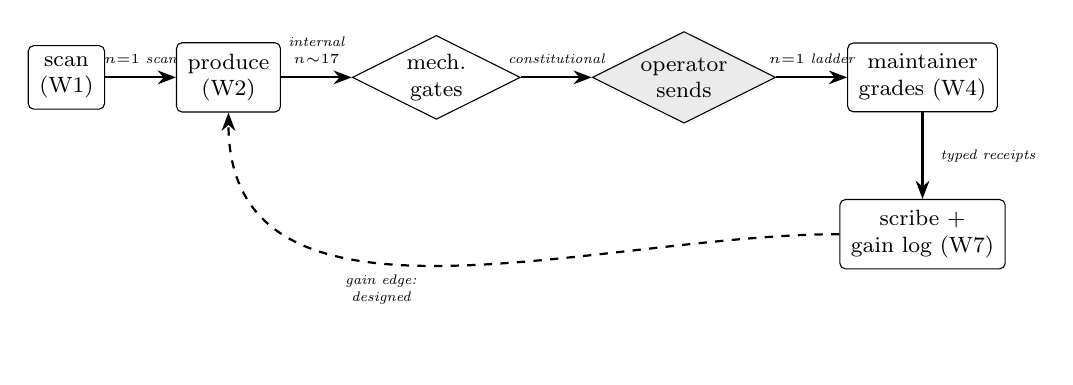
\begin{tikzpicture}[
  every node/.style={font=\footnotesize},
  stage/.style={draw, rectangle, rounded corners=2pt, minimum height=7mm, inner sep=4pt, align=center},
  gate/.style={draw, diamond, aspect=2, inner sep=1pt, align=center},
  wit/.style={-{Stealth}, thick},
  unwit/.style={-{Stealth}, thick, dashed},
  lab/.style={font=\tiny\itshape, align=center}]

\node[stage] (scan) {scan\\(W1)};
\node[stage, right=9mm of scan] (produce) {produce\\(W2)};
\node[gate, right=9mm of produce] (mech) {mech.\\gates};
\node[gate, right=9mm of mech, fill=black!8] (op) {operator\\sends};
\node[stage, right=9mm of op] (world) {maintainer\\grades (W4)};
\node[stage, below=11mm of world] (learn) {scribe +\\gain log (W7)};

\draw[wit] (scan) -- node[lab, above=0.5mm] {$n{=}1$ scan} (produce);
\draw[wit] (produce) -- node[lab, above=0.5mm] {internal\\$n{\sim}17$} (mech);
\draw[wit] (mech) -- node[lab, above=0.5mm] {constitutional} (op);
\draw[wit] (op) -- node[lab, above=0.5mm] {$n{=}1$ ladder} (world);
\draw[wit] (world) -- node[lab, right=1mm] {typed receipts} (learn);
\draw[unwit] (learn.west) to[out=180, in=-90] node[lab, below left=0mm and 2mm] {gain edge:\\designed} (produce.south);
\end{tikzpicture}
\caption{The emission loop. The shaded gate is the constitutional
consent boundary: everything left of it is automatable and
kernel-graded; everything right of it is graded by the world on the
world's clock. The dashed return edge --- review content changing
what gets built --- is the loop's gain (WR-27), instrumented from
birth and not yet witnessed.}
\label{fig:loop}
\end{figure}

\section{The consent gate is a feature of the theorem}
\label{sec:consent}

The APM pipeline's ambition is zero standing human involvement
outside two named judgment checkpoints. This pipeline is different
\emph{by constitution}: outward acts are excluded from autonomous
admissibility, permanently. It matters to say precisely what is and
is not being claimed, because ``automated'' would otherwise be doing
dishonest work: the claim is that \emph{production, gating, tracking,
and learning} run without operator adjudication, while
\emph{emission} is operator-gated by design. The re-arm condition
that governs the WM's overnight running (one cohort scored
end-to-end with zero operator-adjudication events, written at the
switch in \texttt{WM-OVERNIGHT-RUNBOOK.md}) is therefore a condition
on the \emph{scoring} loop, not on the send gate; the two human roles
--- adjudicator (to be engineered away) and sender (to be kept) ---
must not be conflated in either direction. A reviewer who reads the
send gate as an automation failure has been given the wrong theorem;
a builder who automates the send gate to improve a metric has
violated the constitution, not optimized it.

This section is also the series' first demand for a stronger logic:
its content is signalling-shaped, and its proper form --- the send
gate as a one-way-signalling judgment ($A \triangleleft B$ in BV,
where the War Machine is native) --- is registered as tier~D2 of the
companion note \emph{capability-proof-diagramprover}, whose
first-application contract is to type Figure~\ref{fig:loop} as a BV
formula and check the invariants of this section as derivability
facts.

\section{Current warrant state}

\begin{center}
\small
\begin{tabular}{p{0.34\textwidth} p{0.17\textwidth} p{0.36\textwidth}}
\textbf{Sub-claim} & \textbf{Warrant} & \textbf{Key certificates}\\[2pt]
\hline\\[-8pt]
W1 The scan finds honest rungs & inductive-$n{=}1$ & one afternoon's
standing~$\times$~liveness sweep yielded ${\sim}10$ walkable rungs in
3 tiers; drop rule enforced with recorded reasons; a month of staged
sends from one pass\\[3pt]
W2 The relay produces mergeable work & rehearsal only & ${\sim}17$
PRs merged under the internal Tickle pipeline with author${}\neq{}$%
reviewer --- own-repo, so \emph{rehearsal-class}: counts for the
mechanism, not as xeno-evaluation; external merged PRs $n{=}0$\\[3pt]
W3 Emission is consent-gated & mechanical (by construction) &
\texttt{autonomous-admissible?} excludes outward acts; needs-you NAG
seam surfaces them; the \#5637 send was made at the operator's
hand\\[3pt]
W4 The world grades, and grading is captured & inductive-$n{=}1$
(full ladder) & send $\to$ reply (first of any campaign, warm or
cold) $\to$ call held $\to$ collaboration path agreed (\#3663 first,
then a \#5637 benchmark); receipts typed and on file\\[3pt]
W5 The memory loop serves code work & designed & the store, scribe,
hunger audit, and task-frame results transport from the APM proof
(cited, not restated --- including N5's weakness, which is shared);
code-domain instances not yet run\\[3pt]
W6 Capability transports APM $\to$ OSS & designed & formally a
transport claim: the selection diagram's $S$ switches domain
(kernel-graded proof vs.\ maintainer-graded code); the shared
mechanism (relay, boundary artifacts, mechanical gates, memory) must
be separated from the grader before ``solves APM $\Rightarrow$
capable upstream'' is identified\\[3pt]
W7 Outcomes are scoreable at three layers & designed & layered
grader specified (mechanical / social-mechanical / terminal);
gain instrumentation (WR-27) specified; latency economics named
(\S\ref{sec:seq})\\[3pt]
W8 The process learns at the ability level & designed &
contribution-type packet templates (evidence-comment,
maintainer-blessed PR, collaboration entry) as versioned artifacts;
none yet authored\\[3pt]
W9 The loop runs continuously & designed, components hand-run & the
bulletin-13/14 walk of the lane (scan $\to$ stage $\to$ send $\to$
reply $\to$ conversion) is the by-hand run of this loop, exactly as
APM's 08-03 factorial was of its driver; the WM scheduler's
guardrails apparatus is live-verified; the composed driver is not
built\\
\hline
\end{tabular}
\end{center}

\medskip
The shape of this table is the message: two inductive-$n{=}1$
witnesses at the ends of the ladder (discovery works; the world
answers), a rehearsal-class middle, and \warrant{designed}
everywhere else. That is what a naturalistic capability claim looks
like at the start, and the table exists so that its future upgrades
are forced through certificates rather than enthusiasm.

\section{The causal layer, and the sequencing argument}
\label{sec:seq}

Two identification questions matter here; both are stated so the
causal engine can refuse what is not identified.

\textbf{Does the harness cause the merges?} The confounder is
standing: a contributor with warm relationships gets merged more
easily regardless of artifact quality. The design answer is the
layered grader: mechanical-layer outcomes (does it build, does the
bug reproduce, does upstream CI pass) are standing-independent and
harvestable pre-send, so the harness's contribution is measurable
below the confounded layer; and the honest-standing drop rule caps
how much standing the selector is allowed to spend. Social-layer
contrasts (reply rates, review rounds) are observational and will be
labeled as such.

\textbf{Does APM capability transport?} W6 is the modularity claim
of the evaluation harness made formal: the harness fixes cohort
definition, dispatch, receipts, scoring discipline; the setting
supplies problem source and grader. Transport holds exactly insofar
as the mechanism edges (relay $\to$ artifact quality) can be
separated from the grader edge ($S$-dependent). The BPM companion
paper is, among other things, the clean-grader measurement of the
shared mechanism --- which is the formal content of the sequencing
intuition: \emph{the fast incorruptible grader measures the
mechanism; the slow unlaunderable grader measures the value.} Run
them in that order and each covers the other's blind side: BPM
answers ``is the capability real?'' where memorization and statement
fidelity can be controlled; OSS answers ``is it worth anything?''
where no benchmark can be gamed because there is no benchmark.

\section{Honest boundaries}

External merges are $n{=}0$; nothing in this note claims otherwise.
The one full-ladder witness converted to a \emph{collaboration
path}, not yet to merged code. Cadence has already failed once (one
send in thirteen days against a proposed one/week); the ledger says
so. The identity question is load-bearing and unresolved --- standing
accrues to a findable name, and three names currently carry pieces of
it. Two hazards are named before they bite: some upstream projects
have explicit policies restricting AI-generated contributions ---
the scan must check the contribution policy per candidate and the
drop rule extends to ``policy forbids what we would send''; and the
social layer can starve silently (maintainer bandwidth is not ours to
schedule), which is what the \emph{not-yet-answered} species and the
compounding-artifact property of public comments are for. Finally,
the claim's relativity to its selector is permanent: this procedure
proves capability \emph{on rungs the scan honestly claims}, and any
attempt to read it as unconditional upstream competence should be
refused by the reader as it would be by the engine.

\section{What this is for}

The APM note argued that the transferable object is the form: a
programme that states its own capability claim constructively and
upgrades only by certificate. This note adds what the form does when
the grader is a human institution: it splits the grader into layers
so that certificates exist below the confounded ones; it types
silence (\emph{not-yet-answered}) so that a slow world neither
blocks nor flatters the proof; and it locates the consent gate
inside the theorem, so that ``the War Machine works while the
operator sleeps'' and ``the operator sends'' are seen to be
compatible claims --- indeed, the same claim, stated at the two
places where each belongs. The pipeline's next certificates are
already queued by the table: a second scan (W1 replication), the
first external mechanical-layer packet (W2), and the packet
templates (W8) that let a merge, when it comes, teach the next one.

\end{document}
